%; whizzy paragraph -pdf xpdf -latex ./whizzypdfptex.sh
%; whizzy-paragraph "^\\\\begin{frame}\\|\\\\emtext"
% latex beamer presentation.
% platex, latex-beamer でコンパイルすることを想定。 

%     Tokyo Debian Meeting resources
%     Copyright (C) 2012 Junichi Uekawa

%     This program is free software; you can redistribute it and/or modify
%     it under the terms of the GNU General Public License as published by
%     the Free Software Foundation; either version 2 of the License, or
%     (at your option) any later version.

%     This program is distributed in the hope that it will be useful,
%     but WITHOUT ANY WARRANTY; without even the implied warreanty of
%     MERCHANTABILITY or FITNESS FOR A PARTICULAR PURPOSE.  See the
%     GNU General Public License for more details.

%     You should have received a copy of the GNU General Public License
%     along with this program; if not, write to the Free Software
%     Foundation, Inc., 51 Franklin St, Fifth Floor, Boston, MA  02110-1301 USA

\documentclass[cjk,dvipdfmx,12pt]{beamer}
\usetheme{Tokyo}
\usepackage{monthlypresentation}

%  preview (shell-command (concat "evince " (replace-regexp-in-string "tex$" "pdf"(buffer-file-name)) "&")) 
%  presentation (shell-command (concat "xpdf -fullscreen " (replace-regexp-in-string "tex$" "pdf"(buffer-file-name)) "&"))
%  presentation (shell-command (concat "evince " (replace-regexp-in-string "tex$" "pdf"(buffer-file-name)) "&"))

%http://www.naney.org/diki/dk/hyperref.html
%日本語EUC系環境の時
\AtBeginDvi{\special{pdf:tounicode EUC-UCS2}}
%シフトJIS系環境の時
%\AtBeginDvi{\special{pdf:tounicode 90ms-RKSJ-UCS2}}

\newenvironment{commandlinesmall}%
{\VerbatimEnvironment
  \begin{Sbox}\begin{minipage}{1.0\hsize}\begin{fontsize}{8}{8} \begin{BVerbatim}}%
{\end{BVerbatim}\end{fontsize}\end{minipage}\end{Sbox}
  \setlength{\fboxsep}{8pt}
% start on a new paragraph

\vspace{6pt}% skip before
\fcolorbox{dancerdarkblue}{dancerlightblue}{\TheSbox}

\vspace{6pt}% skip after
}
%end of commandlinesmall

\title{東京エリアDebian勉強会}
\subtitle{第103回 2013年8月度}
\author{上川純一}
\date{2013年8月17日}
\logo{
\includegraphics[width=8cm]{image200607/openlogo-light.eps}}

\begin{document}

\begin{frame}
\titlepage{}
\end{frame}

\begin{frame}{設営準備にご協力ください。}
会場設営よろしくおねがいします。
\end{frame}

\begin{frame}{Agenda}
\begin{minipage}[t]{0.45\hsize}
  \begin{itemize}
  \item 注意事項
	\begin{itemize}
	 \item 飲食禁止
	\end{itemize}
   \item 最近あったDebian関連のイベント報告
	\begin{itemize}
        \item 第102回 東京エリアDebian勉強会
        \item Debconf
	\end{itemize}
 \end{itemize}
\end{minipage} 
\begin{minipage}[t]{0.45\hsize}
 \begin{itemize}
  \item Debian Trivia Quiz
  \item 事前課題紹介
 \end{itemize}
\end{minipage}
\end{frame}

\section{イベント報告}
\emtext{イベント報告}

\begin{frame}{第102回 東京エリアDebian勉強会}
\end{frame}

\begin{frame}{Debconf}
\end{frame}

\section{DWN quiz}
\emtext{DWN quiz}
\begin{frame}{Debian 常識クイズ}

  Debian の常識、もちろん知ってますよね?
知らないなんて恥ずかしくて、知らないとは言えないあんなことやこんなこと、
みんなで確認してみましょう。

今回の出題範囲は\url{debian-devel-announce@lists.debian.org},
\url{debian-devel@lists.debian.org} に投稿された
内容とDebian Project Newsなどからです。

\end{frame}

\subsection{問題}
 %; whizzy-master ../debianmeetingresume201308.tex
% 以上の設定をしているため、このファイルで M-x whizzytex すると、whizzytexが利用できます。
%

\santaku
{Sylvestre Ledru が JDK についてアナウンスしたのは}
{OpenJDK7にきりかえ}
{JDK6の削除}
{JDK8への移行}
{A}
{java-commonをOpenJDK 7 に切り替えるそうですよ、しかし一部のアーキテクチャ
はOpenJDK 6のまま。}

\santaku
{OpenJDK7でサポートされていないアーキテクチャはどれか}
{mipsel}
{amd64}
{i386}
{A}
{s390, mips, mipsel, kfreebsd, sparcがサポートされていないようです。}

\santaku
{Summer Of Code のコーディネーションメンバーでないのは誰か}
{David Bremner}
{Nicolas Dandrimont}
{Nobuhiro Iwamatsu}
{C}
{例年Summer of code スポンサーで開発する内容を調整するボランティアがいま
す。}

\santaku
{Brian GuptaがDebianのトレードマークとしてUSPTOに追加登録しようと提案したのは何か}
{ロゴ}
{Debianの文字列}
{DD}
{A}
{`Debian' は登録されていたがロゴは登録されていなかったので登録することに
したようです。}



\section{事前課題}
\emtext{事前課題}

{\footnotesize
 
\begin{prework}{ Yoshida Shin }

VPN を構築した事は有りません。
また、プライベートでも使用した事は有りません。

VPN は仕事で以下の 2個の使い方をしています。
\begin{enumerate}
 \item  データセンターのサーバーにログインする
 \item  緊急対応のため、自宅から職場につなぐ
\end{enumerate}

でも、緊急対応は行わないで済むようにするべきだし、
(緊急対応が無いと仮定すれば、)多くの場合はデータセンターへの接続も
職場からの IP 制限だけで十分だと考えています。

VPN は万一の為に用意するものであり、
あまり積極的に使いたいと思わないです。
\end{prework}

\begin{prework}{ 吉野(yy\_{}y\_{}ja\_{}jp) }

個人的には使ってません.
\end{prework}

\begin{prework}{ sakai }

今のところVPNは利用していない。
そのうち、外出した時用にVPNで自宅とつなごうかなー、ということを考える程度。
\end{prework}

\begin{prework}{ 野島 貴英 }

以前、苦肉の策で2つの拠点間をインターネット経由でopenvpn使って一時的にLANを組み、複数のWEBサイトのWEB-DB間のアクセスを遠方のDBに常時流し込みつづけてそのまま半月ぐらいサービス維持した事があります。使った結果ですが、予想外にも、簡単/大変タフ/非常に安定したVPN経路が組めた記憶があります。ただ、ちゃんとしたデータ取ってないので、感想以上の事がいえない状況ではあります。
\end{prework}

\begin{prework}{ dictoss(杉本 典充) }

最近自宅サーバにopenvpnを入れて、出先でテザリングをしながらサーバにアクセスしている。
それまではsshとポートフォワードでがんばっていたが、サーバの台数が増えるとポートフォワードの数が増えるので設定が疲れました。
VPSから自宅サーバにVPNセッションを張ろうかと思っているが自宅サーバはDynamicDNSを利用しているので切れずにつながっていられるか不明。

会社だと拠点間をつなぐためにL2TP/IPsecでVPNを張る場合や、グロバールIPを持たない(=NAT配下)に設置されるが管理上サーバからsshする必要があるPCにはクライアントからVPNを張らせることでsshできるようにする、といった使い方をしている。
\end{prework}

\begin{prework}{ まえだこうへい }

会社環境に繋ぐのに、OpenVPNと、Cisco Anycoonect を使ってますが、後者の環境では、Anyconnectクライアントではなく、OpenConnectを使ってます。RSA OneTimePasswordのモジュールを併用して二要素認証にしていますが、これにも対応してます。

個人環境ではSSHのProxy機能を使っているので、接続先ノード数増えても特に困らずVPNって面倒だよなぁとふと思い出しながら仕事してます。
\end{prework}

}

\section{openvpn}
\emtext{openvpn}

\begin{frame}{OpenVPNでやりたいこと}
  \includegraphics[width=0.9\hsize]{image201308/network.eps}
\end{frame}

\begin{frame}[containsverbatim]{インストール}
\begin{commandline}
 # apt-get install openvpn openssl
\end{commandline}
\end{frame}

\begin{frame}[containsverbatim]{疎通試験}
\begin{commandline}
 server$ sudo openvpn --dev tun1  \
    --ifconfig 10.1.1.1 10.1.1.2 
 client$ sudo openvpn --dev tun1  \
    --remote サーバホスト名 --ifconfig 10.1.1.2 10.1.11
\end{commandline}
\end{frame}

\begin{frame}[containsverbatim]{CA}
 \begin{commandline}
 # cd /etc/openvpn
 # sudo cp -R /usr/share/doc/openvpn/examples/easy-rsa/2.0/ easy-rsa/
 # cd easy-rsa/
 # vi vars
 # . ./vars
 # ./clean-all
 # ./build-ca

\end{commandline}
\end{frame}

\begin{frame}[containsverbatim]{サーバー鍵の作成と設定の作成}

\begin{commandline}
 # ./build-key-server sakura
 # ./build-dh  
\end{commandline}

\end{frame}

\begin{frame}[containsverbatim]{クライアント鍵の作成}
\begin{commandline}
 # ./build-key client1
 # ./build-key nexus4
\end{commandline}
\end{frame}

\begin{frame}[containsverbatim]{HMAC鍵の作成}
\begin{commandline}
 # openvpn --genkey --secret ta.key
\end{commandline}
\end{frame}

\begin{frame}[containsverbatim]{server設定の作成}

/etc/openvpn/server.conf を作成して /etc/init.d/openvpn restart

\begin{commandline}
port 1194
proto udp
dev tun
user nobody
group nogroup
tls-auth      /etc/openvpn/easy-rsa/keys/ta.key 0 # server is 0.
ca      /etc/openvpn/easy-rsa/keys/ca.crt
cert    /etc/openvpn/easy-rsa/keys/sakura.crt
key     /etc/openvpn/easy-rsa/keys/sakura.key  # keep secret
dh      /etc/openvpn/easy-rsa/keys/dh1024.pem
server 10.55.2.0 255.255.255.0  # internal tun0 connection IP
ifconfig-pool-persist ipp.txt
keepalive 10 120
comp-lzo         # Compression - must be turned on at both end
persist-key
persist-tun
status log/openvpn-status.log
verb 3  # verbose mode
client-to-client
 
\end{commandline}
\end{frame}

\begin{frame}{topology net30}

/30 の ipv4 アドレスネットワークをクライアントごとに作成。4IPアドレスを
消費。

\end{frame}

\begin{frame}{tun/tap}

\begin{tabular}{|c|p{4em}|p{8em}|p{8em}|}
\hline
 & ネットワークレイヤー & 機能 & つかえるOS\\
\hline
tap & L2 & ブリッジ(ブロードキャストパケットが到達する) & linux \\
tun & L3 & ルータ & linux, iOS, Androidなど \\
\hline
\hline
\end{tabular}
\end{frame}

\begin{frame}[containsverbatim]{クライアント側の設定}
\url{/etc/openvpn/*.conf}においておけば勝手にネットワークに変更があれば
 実行される設定になっています。

\begin{commandline}
client
dev tun
port 1194
proto udp
remote xyz.sakura.ne.jp 1194
nobind
tls-auth      ta.key 1 # client is 1.
ca ca.crt
cert android-nexus4.crt
key android-nexus4.key
remote-cert-tls server
comp-lzo
persist-key
persist-tun
verb 3
\end{commandline}
\end{frame}

\begin{frame}[containsverbatim]{Androidにインポート 0}
ファイルをコピー
\begin{commandline}
$ ls -1 
android-nexus4.crt
android-nexus4.csr
android-nexus4.key
ca.crt
client.ovpn
ta.key
$ adb push . /sdcard/secure
push: ./ca.crt -> /sdcard/secure/ca.crt
push: ./android-nexus4.key -> /sdcard/secure/android-nexus4.key
push: ./ta.key -> /sdcard/secure/ta.key
push: ./android-nexus4.crt -> /sdcard/secure/android-nexus4.crt
push: ./client.ovpn -> /sdcard/secure/client.ovpn
push: ./android-nexus4.csr -> /sdcard/secure/android-nexus4.csr
\end{commandline}
\end{frame}

\begin{frame}{Androidにインポート 1}

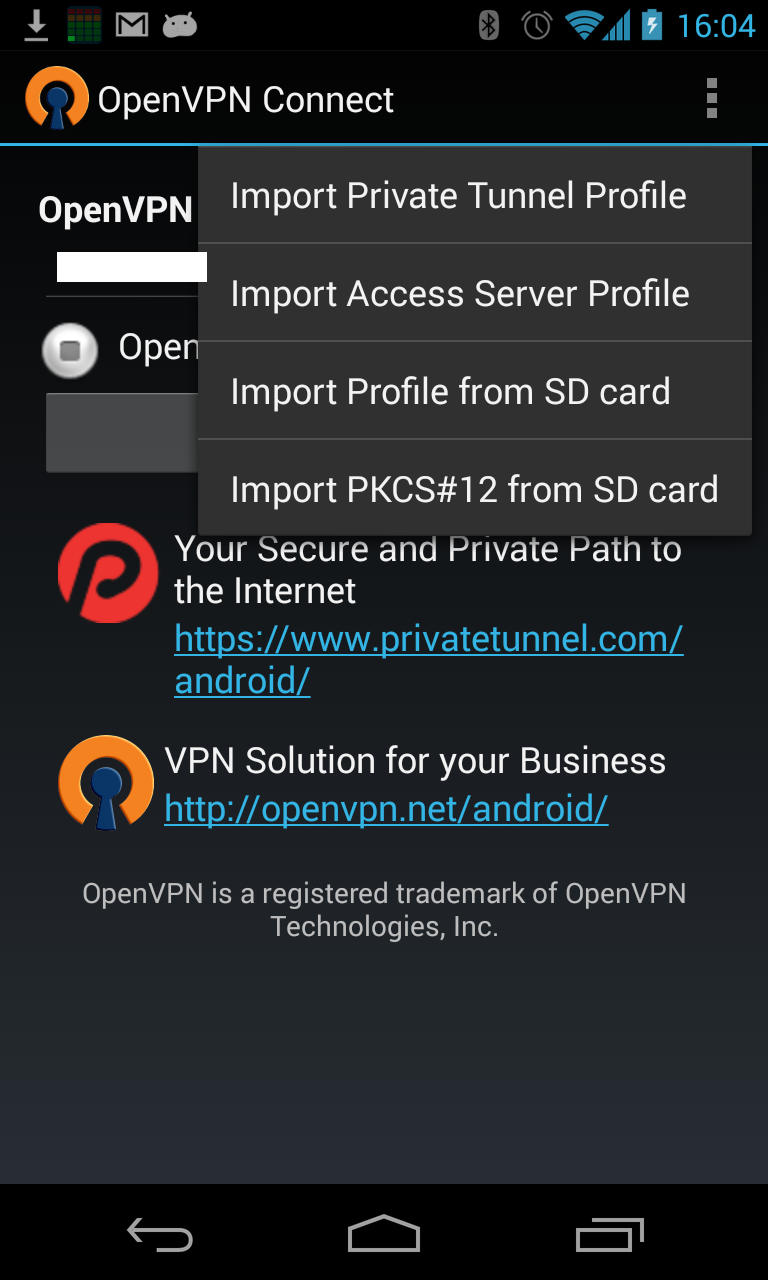
\includegraphics[height=0.9\vsize,bb=0 0 768 1280]{image201308/Screenshot_2013-08-17-16-04-31.png}

\end{frame}
\begin{frame}{Androidにインポート 2}
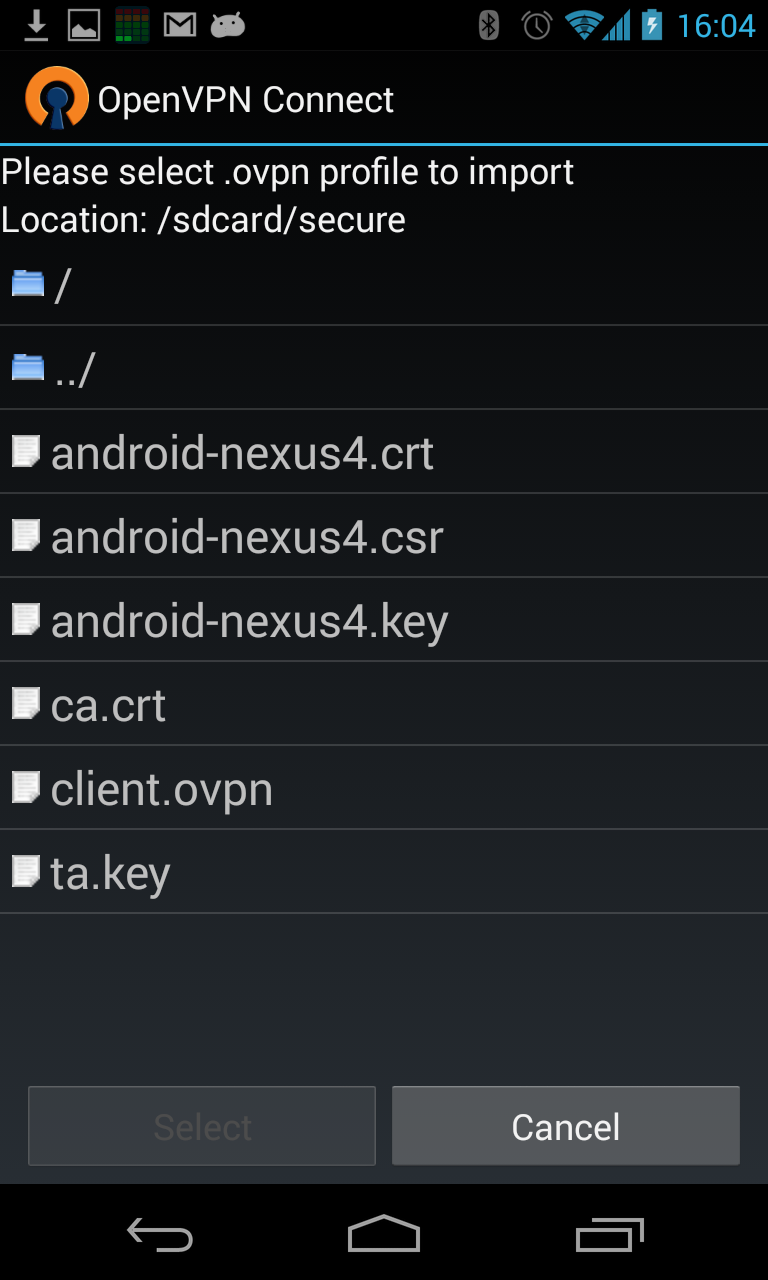
\includegraphics[height=0.9\vsize,bb=0 0 768 1280]{image201308/Screenshot_2013-08-17-16-04-43.png}

\end{frame}
\begin{frame}{Androidにインポート 3}
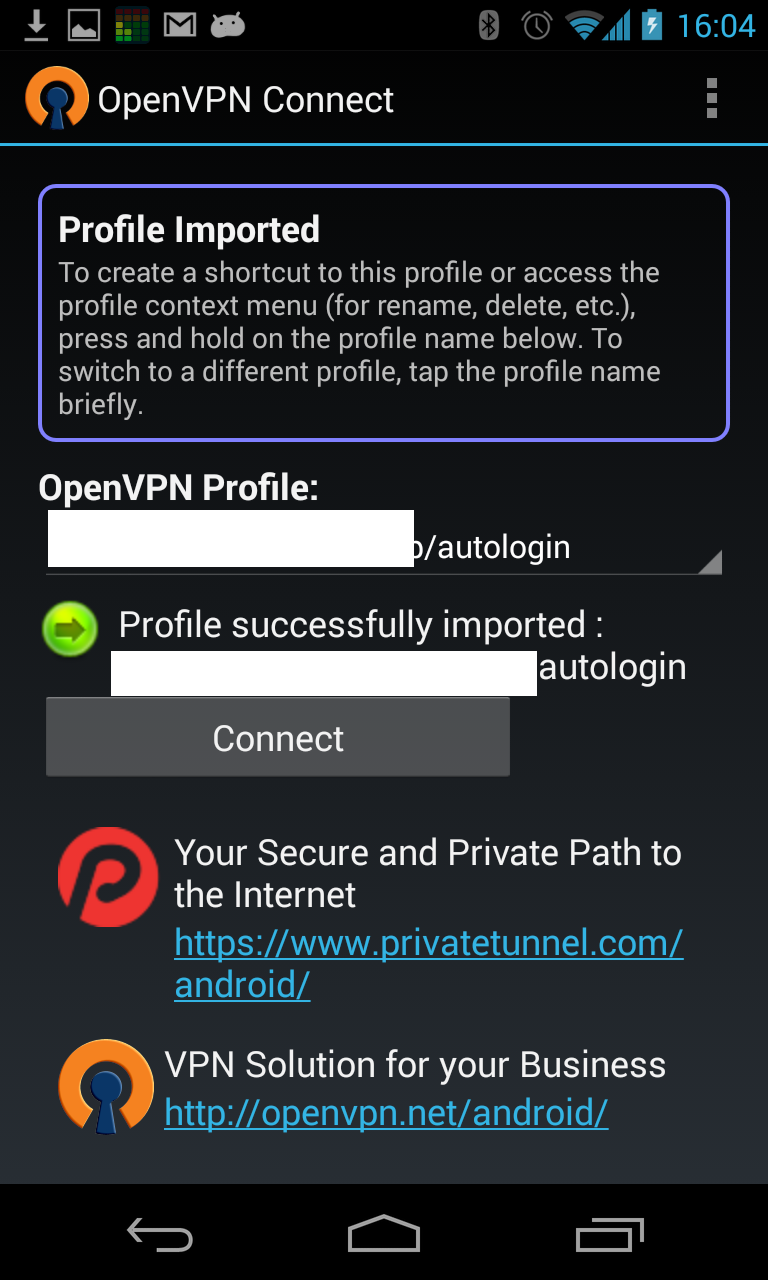
\includegraphics[height=0.9\vsize,bb=0 0 768 1280]{image201308/Screenshot_2013-08-17-16-04-54.png}

\end{frame}
\begin{frame}{Androidにインポート 4}
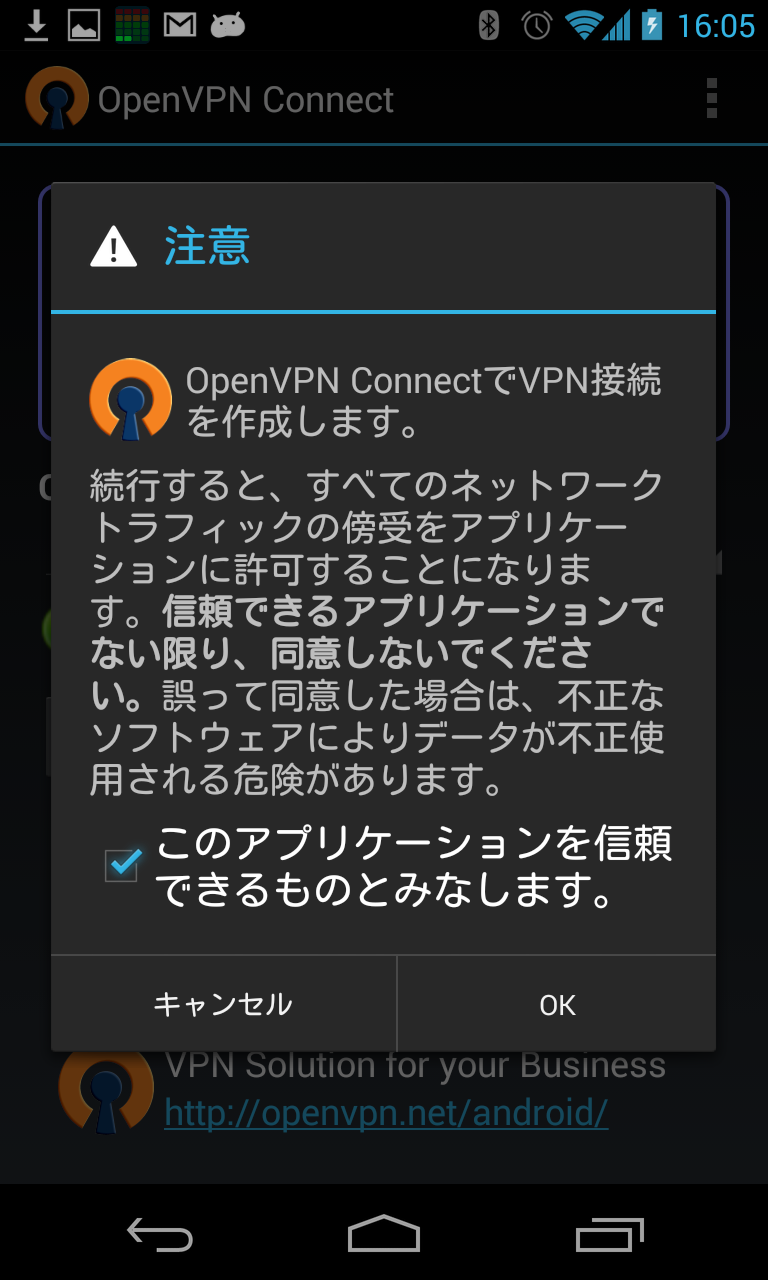
\includegraphics[height=0.9\vsize,bb=0 0 768
 1280]{image201308/Screenshot_2013-08-17-16-05-07.png}
\end{frame}

\begin{frame}{Androidにインポート}
これでディレクトリ削除してよいです。
\end{frame}

\begin{frame}{一方sshは}
 
\begin{table}[H]
 \caption{ssh の機能の対応}
 \begin{tabular}{|p{6em}|p{8em}|p{10em}|}
 \hline
 & sshオプション & 機能 \\
 \hline
 ポートフォワーディング &  -L, -R & 特定のローカルのTCPポート番号をリモートのポート番
	 号とマッピングする \\
 \hline
 プロキシ & -D & SOCKSに対応しているアプリケーションのプロキシを提供 \\
 \hline
 VPN & -w & IPレベルで相互に見えるよう仮想的にネットワークを構築する \\
 \hline
 \hline
 \end{tabular}
\end{table}

\end{frame}


\section{epub}
\emtext{epub}

\section{今後のイベント}
\emtext{今後のイベント}
\begin{frame}{今後のイベント}
\begin{itemize}
 \item 2013年9月 Debian勉強会
\end{itemize}
\end{frame}

\section{今日の宴会場所}
\emtext{今日の宴会場所}
\begin{frame}{今日の宴会場所}
未定
\end{frame}

\end{document}

;;; Local Variables: ***
;;; outline-regexp: "\\([ 	]*\\\\\\(documentstyle\\|documentclass\\|emtext\\|section\\|begin{frame}\\)\\*?[ 	]*[[{]\\|[]+\\)" ***
;;; End: ***
